\documentclass{article}
% \usepackage{showframe}
\usepackage{siunitx}
\usepackage{booktabs}
\usepackage{graphicx}
% \usepackage{minted}

\frenchspacing
\setlength{\parindent}{0ex}
\setlength{\parskip}{3 ex plus 2 ex minus 1 ex}

\title{Homework 3}
\author{Josh Bradt}
\date{February 8, 2016}

\begin{document}

\maketitle

The timing results for each transpose method are shown in Table~\ref{tab:results}. These results are also plotted in Figure~\ref{fig:resloglog}.

In all cases, the cache oblivious code produced the fastest transpose times, though it was still slower than the prediction from the model by a factor of around 4 to 8. For small matrices, the basic transpose outperformed the blocked transpose, but for large matrices, the blocked transpose was faster. This is likely an effect of the extra overhead of the blocked transpose.

The model I used for the prediction was
\begin{equation}
    \text{time} = C N^2
\end{equation}
where $C$ is the copy time from STREAM, and $N$ is the size of the matrix. The copy time I had gotten from STREAM was \SI{3.141}{ms} for \num{3000000} elements, so I used a value of $C = (\SI{3.141}{ms}) / (\SI{3000000}{elements}) = \SI{1.047}{ns/element}$.

\begin{table}[b]
\centering
\begin{tabular}{S[table-format=4]
                S[table-format=2.3e+2]
                S[table-format=2.3e+2]
                S[table-format=2.3e+2]
                S[table-format=2.4e+2]}
\toprule
{Size} & {Basic {[}s{]}} & {Model {[}s{]}} & {Blocked {[}s{]}} & {Cache Oblivious {[}s{]}} \\ \midrule
20   & 9.537E-07     & 4.188E-07     & 1.907E-06      & 1E-06                   \\
100  & 2.790E-05     & 1.047E-05     & 4.101E-05      & 2.9E-05                 \\
500  & 1.059E-03     & 2.618E-04     & 1.037E-03      & 8.49E-04                \\
1000 & 8.120E-03     & 1.047E-03     & 4.880E-03      & 4.93E-03                \\
1500 & 1.828E-02     & 2.356E-03     & 1.147E-02      & 1.0964E-02              \\
2000 & 3.969E-02     & 4.188E-03     & 2.061E-02      & 2.0465E-02              \\
4000 & 1.978E-01     & 1.675E-02     & 8.718E-02      & 8.699E-02               \\ \bottomrule
\end{tabular}
\caption{Transpose timing results. The basic and blocked codes were written to run 11 iterations for each array size. The first of these iterations was thrown out to avoid cold start effects, and then the minimum time from the remaining 10 iterations was recorded in this table.}
\label{tab:results}
\end{table}

\begin{figure}
    \centering
    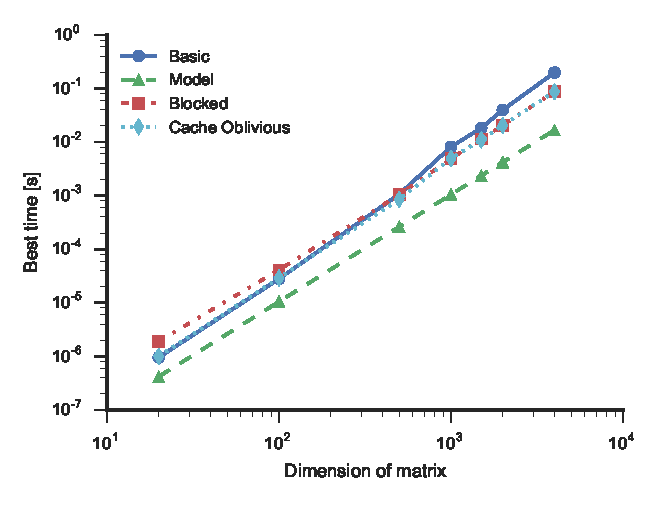
\includegraphics{res_loglog.pdf}\hspace{0.9cm}
    \caption{A plot of the results on a log-log scale.}
    \label{fig:resloglog}
\end{figure}

\end{document}
